\subsection{2.2~~线性表的顺序存储}
\begin{frame}\ft{\subsecname}
\begin{dingyi}[顺序存储 Sequence List]
把结点按逻辑顺序依次存放在一组地址连续的存储单元里. 
以这种方式存储的线性表简称顺序表. 
\end{dingyi}

\pause 
\begin{block}{特点}
\begin{itemize}
\item
逻辑顺序与物理顺序一致;
\item
数据元素之间的关系是以元素在计算机内“物理位置相邻”来体现的. 
\end{itemize}
\end{block}
\end{frame}

\begin{frame}\ft{\subsecname}
  设有非空线性表$(a_1,a_2,\cd,a_n)$,  $l_i$表示$a_i$的存储位置,  $k$为每个元素需占用的存储单元. 
\begin{figure}
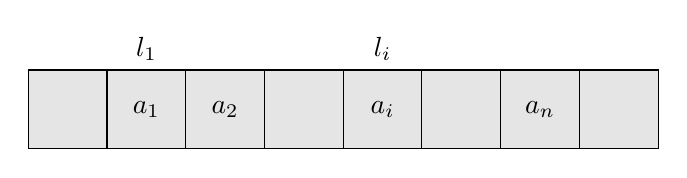
\begin{tikzpicture}
\foreach \i in {1,...,8}
\filldraw[fill=black!10] (\i-1,0)rectangle(\i,1);
\node [] at (0.5,0.5) {$\cd$};
\node [] at (1.5,0.5) {$a_1$}; \node [above] at (1.5,1) {$l_1$}; 
\node [] at (2.5,0.5) {$a_2$};
\node [] at (3.5,0.5) {$\cd$};
\node [] at (4.5,0.5) {$a_i$}; \node [above] at (4.5,1) {$l_i$}; 
\node [] at (5.5,0.5) {$\cd$};
\node [] at (6.5,0.5) {$a_n$};
\node [] at (7.5,0.5) {$\cd$};
\end{tikzpicture}
\caption{线性表的顺序存储}
\end{figure}


%第$i+1$个数据元素的存储位置$Loc(a_{i+1})$和第$i$个数据元素的存储位置$Loc(a_{i})$之间满足
$$
l_{i+1}=l_{i}+k
$$
%其中$l$为线性表每个元素需占用的存储单元. 特别地,  
$$
l_{i}=l_{1}+(i-1)k
$$
\end{frame}

\begin{frame}[fragile]\ft{\subsecname}
\begin{lstlisting}[title=顺序存储的结构代码,language=C,frame=tb,backgroundcolor=\color{red!10}]
#define MAX_SIZE 100
typedef int ElemType;
typedef struct sqlist {
    ElemType data[MAX_SIZE];
    int length;
}
\end{lstlisting}


%% \begin{itemize}
%% \item 存储空间的起始位置: 数组{\ttfamily elem\_array}, 其存储位置就是存储空间的存储位置
%% \item 线性表的最大存储容量: 数组长度{\ttfamily MAX\_SIZE}
%% \item 线性表的当前长度: {\ttfamily length}
%% \end{itemize}
\end{frame}

\begin{frame}\ft{\subsecname}
  \begin{zhu}[数据长度与线性表长度的区别]
    \begin{itemize}
    \item 数组长度是存放线性表存储空间的长度,存储分配后一般不变; 
    \item 线性表长度是线性表中数据元素的个数,随着线性表插入和删除操作的进行而发生变化; 
    \item 线性表长度总小于等于数组长度。
    \end{itemize}
  \end{zhu}
\end{frame}

\begin{frame}\ft{\subsecname}\fst{基本操作}
\begin{itemize}
\item
初始化
\item
赋值
\item
查找
\item
修改
\item
插入
\item
删除
\item
求长度
\item
$\cd$
\end{itemize}•
\end{frame}


\begin{frame}[fragile]\ft{\subsecname}\fst{基本操作}
  \begin{lstlisting}[frame=tb,language=C]
#define OK 1
#define ERROR 0
#define TRUE 1
typedef int Status;
  \end{lstlisting}
\end{frame}

\begin{frame}[fragile]\ft{\subsecname}\fst{基本操作(初始化)}
\begin{lstlisting} [language=C,frame=tb,backgroundcolor=\color{red!10}]
Status SqListInit(SqList *L) {
  L->data=(ElemType *) malloc(MAX_SIZE*sizeof(ElemType));
  if(!L->data) return ERROR;
  L->length=0;
  return OK;
}
\end{lstlisting}

\end{frame}

\begin{frame}[fragile]\ft{\subsecname}\fst{基本操作(插入结点)}
\begin{block}{目标}
在$L=(a_1,\cd,a_{i-1},\red{a_i},a_{i+1},\cd,a_n)$中的第$i$个位置上插入新结点$e$,  使其成为
$$
L=(a_1,\cd,a_{i-1},e,a_i,a_{i+1},\cd,a_n)
$$
\end{block}
\pause 
\begin{block}{实现步骤}
\begin{itemize}
\item
  如果插入位置不合理,抛出异常;
\item
  如果线性表长度大于等于数组长度,抛出异常或动态增加容量;
\item
  从最后一个元素开始向前遍历到第$i$个位置,分别将它们向后移动一个位置;
\item
  将元素{\ttfamily e}填入位置{\ttfamily i}处;
\item
线性表长度加1.
\end{itemize}
\end{block}

\end{frame}

\begin{frame}[fragile]\ft{\subsecname}\fst{基本操作(插入结点)}
\begin{lstlisting} [language=C,breaklines,backgroundcolor=\color{red!10},frame=tb]
Status SqListInsert(SqList *L,int i,ElemType e){
  int j;
  if (L->length>=MAX_SIZE) { //`线性表已满`
    printf("`线性表溢出!`\n"); return ERROR;
  }
  if (i<0||i>L->length-1)   //`i不在范围内`
    return ERROR;
  for (j=L->length-1; j>=i-1; j--)
    L->data[j+1]=L->data[j];
  L->data[i-1]=e;
  L->length++;
  return OK;
}
\end{lstlisting}

\end{frame}

\begin{frame}\ft{\subsecname}\fst{基本操作(插入结点)}
在{\ttfamily L}的第$i$个元素之前插入新结点,  其时间主要耗费在结点的移动上. 因此,  可用结点的移动来估计算法的时间复杂度. \vspace{0.1in}

设在{\ttfamily L}的第$i$个元素之前插入结点的概率为$p_i$. 不失一般性,  设各位置插入等概率,  则$p_i=\frac1{n+1}$,  而插入时移动结点的次数为$n-i+1$,  故总的平均移动次数为
$$
E_{insert}=\sum_{i=1}^n p_i (n-i+1)=\frac n2.
$$\vspace{0.1in}

这表明,  在顺序表上做插入运算,  平均要移动表上一半的结点. 当表长$n$较大时,  算法效率相当低. 因此算法的平均时间复杂度为$O(n)$. 
\end{frame}

\begin{frame}\ft{\subsecname}\fst{基本操作(删除结点)}
\begin{block}{目标}
在
$$
L=(a_1,\cd,a_{i-1},\red{a_i},a_{i+1},\cd,a_n)
$$
中删除结点$a_i$,  使其成为 
$$
L=(a_1,\cd,a_{i-1},a_{i+1},\cd,a_n)
$$
\end{block}
\pause 
\begin{block}{实现步骤}
\begin{itemize}
\item
  若删除位置不合理,跑出异常;
\item
  取出删除元素;
\item
  从删除元素的位置开始遍历到最后一个元素的位置,分别将它们向前移动一个位置;
\item
  表长减1.
\end{itemize}
\end{block}
\end{frame}


\begin{frame}[fragile]\ft{\subsecname}\fst{基本操作(删除结点)}
\begin{lstlisting} [language=C,breaklines,backgroundcolor=\color{red!10},frame=tb]
Status SqListDelete(SqList *L,int i,ElemType *e) {
  int j; 
  if (L->length==0) {
    printf("`线性表为空!`\n"); return ERROR;
  }
  if (i<0||i>L->length)  {
    printf("`要删除的数据元素不存在!`\n"); 
    return ERROR;
  }
  else {
    *e=L->data[i-1];
    for (j=i; j<L->length; j++)
      L->data[j-1]=L->data[j];
    L->length--;
    return OK;
  }
}
\end{lstlisting}

\end{frame}


\begin{frame}\ft{\subsecname}\fst{基本操作(删除结点)}
删除{\ttfamily L}的第$i$个元素,  其时间主要耗费在表中结点的移动操作上. 因此,  可用结点的移动来估计算法的时间复杂度. \vspace{0.1in}

设在{\ttfamily L}中删除第$i$个元素的概率为$p_i$,  不失一般性,  设各个位置插入等概率,  则$p_i=\frac1{n}$,  而插入时移动结点的次数为$n-i$,  故总的平均移动次数为
$$
E_{delete}=\sum_{i=1}^n p_i (n-i)=\frac {n-1}2.
$$\vspace{0.1in}

这表明,  在顺序表上做删除运算,  平均要移动表上一半的结点. 当表长$n$较大时,  算法效率相当低. 因此算法的平均时间复杂度为$O(n)$. 
\end{frame}

\begin{frame}\ft{\subsecname}\fst{基本操作(查找、定位删除)}
\begin{block}{目标}
在$L=(a_1,a_2,\cd,a_n)$中删除值为$x$的第一个结点. 
\end{block}
\pause 
\begin{block}{实现步骤}
\begin{itemize}
\item[(1)]
在{\ttfamily L}中查找值为$x$的第一个数据元素;
\item[(2)]
将从找到的位置至最后一个结点依次向前移动一个位置;
\item[(3)]
线性表长度减1. 
\end{itemize}
\end{block}
\end{frame}


\begin{frame}[fragile]\ft{\subsecname}\fst{基本操作(查找、定位删除)}
\begin{lstlisting} [language=C,breaklines,backgroundcolor=\color{red!10},frame=tb]
Status SqListLocateDelete(SqList *L,ElemType x) {
  int i=0,k;
  while (i<L->length){
    if (L->data[i]!=x) i++;
    else {
      for (k=i+1;k<L->length;k++)
        L->data[k-1]=L->data[k];
      L->length--; break;
    }
  }
  if (i>L->length) {
    printf("要删除的数据元素不存在!\n");
    return ERROR;
  }
  return OK;
}
\end{lstlisting}

\end{frame}

\begin{frame}\ft{\subsecname}\fst{基本操作(查找、定位删除)}
时间主要耗费在数据元素的比较和移动操作上. \vspace{0.1in}

 
设在{\ttfamily L}中删除数据元素的概率为$p_i$,  不失一般性,  设各个位置等概率,  则$p_i=\frac1{n}$. 
\begin{itemize}
\item 比较的平均次数为:
$$
E_{compare} = \sum_{i=1}^n p_i i= \frac{n+1}2
$$
\item 删除时的平均移动次数为
$$
E_{delete} =\sum_{i=1}^n p_i (n-i)=\frac {n-1}2.
$$\
\end{itemize}•
平均时间复杂度为
\[
E_{compare}+E_{delete}=n
\]

\end{frame}


\begin{frame}\ft{\subsecname}\fst{顺序表的优缺点}
  \begin{block}{优点}
    \begin{itemize}
    \item 无须为表示表中元素之间的逻辑关系而增加额外的存储空间
    \item 可以快速地存取表中任一位置的元素
    \end{itemize}
  \end{block}

  \pause

  \begin{block}{缺点}
    \begin{itemize}
    \item 插入和删除操作需要移动大量元素
    \item 当线性表变化较大时,难以确定存储空间的容量
    \item 造成存储空间的“碎片”
    \end{itemize}
  \end{block}


\end{frame}
